\chapter{Conceptos teóricos}
\label{chap:conceptos}


\lettrine{E}{}n este capítulo se abordan los conceptos fundamentales necesarios para la realización de este \acrfull{TFG}.

\section{Modelos de lenguaje masivos}

Los \acrfull{LLMs} son un tipo de modelos de inteligencia artificial que utiliza técnicas de aprendizaje automático para comprender y producir lenguaje humano. Estas herramientas pueden ser de gran utilidad para las compañías y organizaciones que desean automatizar y mejorar diferentes áreas de la comunicación y del análisis de datos.

Los \acrshort{LLMs} utilizan modelos basados en redes neuronales y técnicas de \acrfull{NLP} para procesar y estimar sus resultados. El \acrshort{NLP} es un campo de la inteligencia artificial que se centra en lograr que las computadoras comprendan, interpreten y generen texto. Esto, a su vez, permite que los \acrshort{LLMs} realicen diversas tareas: analizar texto y sentimientos u opiniones, traducir idiomas y reconocer voces.

Los \acrshort{LLMs}, como \acrfull{GPT} y \acrfull{LLaMA}, utilizan un método conocido como aprendizaje no supervisado para comprender y procesar el lenguaje natural. En este proceso, se proporcionan extensos conjuntos de datos al modelo, que los analiza y aprende de forma autónoma a través de ejemplos sin etiquetar previamente. Esta fase de preentrenamiento es crucial para desarrollar la capacidad del modelo de generar respuestas coherentes y contextualmente adecuadas sin supervisión directa.

Debido a la necesidad de realizar cálculos constantes de probabilidades para encontrar conexiones, \acrshort{LLMs} requieren una cantidad significativa de recursos computacionales. Las \acrfull{GPU}s son uno de los recursos utilizados para obtener potencia informática. Las \acrshort{GPU}s son dispositivos  especializados de hardware diseñados para gestionar tareas complejas de procesamiento paralelo, lo que hace que sean ideales para los modelos de aprendizaje automático y aprendizaje profundo que requieren realizar numerosos cálculos.

\subsection{Aprendizaje Profundo}

La técnica de inteligencia artificial conocida como aprendizaje profundo consiste en enseñar a las computadoras a procesar datos utilizando algoritmos que se inspiran en el cerebro humano. Este método, denominado aprendizaje profundo o redes neuronales profundas \cite{IBM}, posibilita que las computadoras aprendan mediante la observación, similar a los seres humanos.

Las \acrfull{ANN} son la base del aprendizaje profundo y se basan en el funcionamiento de las neuronas biológicas, pero utilizan neuronas artificiales formadas por nodos de software, como se muestra en la figura \ref{fig:2_Deep Neuronal Network}. Los nodos se valen de operaciones matemáticas (en vez de procesos químicos como el cerebro) para intercambiar y transferir datos en el sistema.

\begin{figure}[hp!]
  \centering
  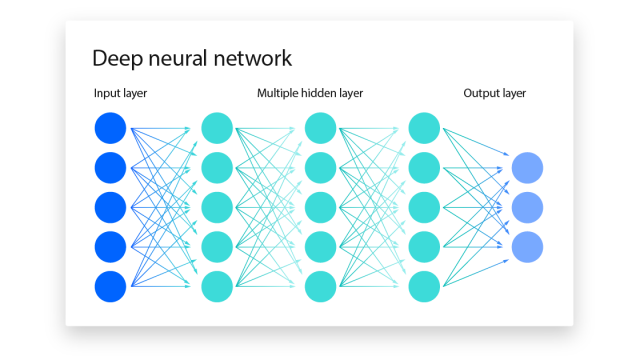
\includegraphics[width=0.75\textwidth]{imaxes/2_Deep Neuronal Network.png}
\caption[Esquema de una Red Neuronal Profunda]{Esquema de una Red Neuronal Profunda. \textit{Fuente: \cite{ResearchGate2024}}}
  \label{fig:2_Deep Neuronal Network}
\end{figure}

\subsection{IA Generativa}
\label{subsec:iagenerativa}


La inteligencia artificial generativa (\acrshort{GenAI}) \cite{IAGenerativa} representa una faceta de la inteligencia artificial que se especializa en la creación de nuevo contenido a través de modelos de aprendizaje profundo. Estos modelos son diferenciados por su habilidad de producir \textbf{ información innovadora} y \textbf{única}, en contraste con los modelos de IA discriminativa, los cuales se centran en la clasificación o distinción entre datos ya existentes. La inteligencia artificial generativa se aprovecha de grandes bases de datos para devolver salidas de calidad, las cuales son creaciones originales que imitan las características de los datos iniciales.

La versatilidad de la \acrshort{GenAI} se demuestra en sus diferentes usos, como la creación de textos, imágenes, y código de software, además de su aplicación en la investigación científica. ChatGPT, DALL-E, GitHub CoPilot \ref{chap:estadodelarte} son algunos de los ejemplos más reconocidos de la \acrlong{GenAI}.
Estos modelos funcionan a través de algoritmos de aprendizaje profundo que generan representaciones codificadas de los datos en los que fueron entrenados, siendo estas representaciones simplificaciones que posibilitan la creación de nueva información manteniendo la esencia de los datos originales. El procedimiento incluye la utilización de métodos como el refinamiento supervisado y la optimización específica para cada situación, garantizando que el resultado sea adecuado para el usuario.

Aunque tiene beneficios, la \acrlong{GenAI} presenta importantes desafíos, especialmente en el ámbito ético y de la seguridad. Contar con la habilidad de crear contenido realista puede resultar en la producción de información falsa o contenido inadecuado, por lo que se necesita un fuerte marco ético y medidas de seguridad sólidas para reducir estos peligros.

\subsubsection{Transformers}
\label{subsubsec:transformers}

Los Transformers son una variedad de \acrfull{DNN} que resuelven los problemas de las arquitecturas secuencia a secuencia, como la dependencia corta de las secuencias de entrada y el procesamiento secuencial, lo que dificulta el entrenamiento en paralelo. Los transformadores \cite{bender2022generacion} utilizan el mecanismo de \textbf{autoatención de múltiples cabezales} para extraer atributos y tienen un alto potencial para usarse en \acrshort{NLP}. En contraste con las técnicas convencionales de recurrencia, Transformers emplean la atención para entender todo un fragmento de una secuencia, mediante bloques de codificación y decodificación, como podemos observar en la figura \ref{fig:2_Transformer}.

La habilidad de Transformers para capturar el verdadero significado del contexto es una ventaja fundamental sobre \acrfull{LSTM} y  \acrfull{RNN}, gracias a su mecanismo de atención. Igualmente, los Transformers son veloces porque tienen la capacidad de operar simultáneamente, a diferencia de las redes recurrentes, y son capaces de aprovechar \acrshort{GPU}, lo que resulta en una ejecución más rápida de tareas que tienen entradas extensas. Los beneficios del modelo Transformer han motivado a expertos del aprendizaje profundo a investigar su utilidad en distintas áreas y ha generado numerosas publicaciones y la creación de modelos basados en Transformer para diversas funciones en inteligencia artificial.

\begin{figure}[!htb]
  \centering
  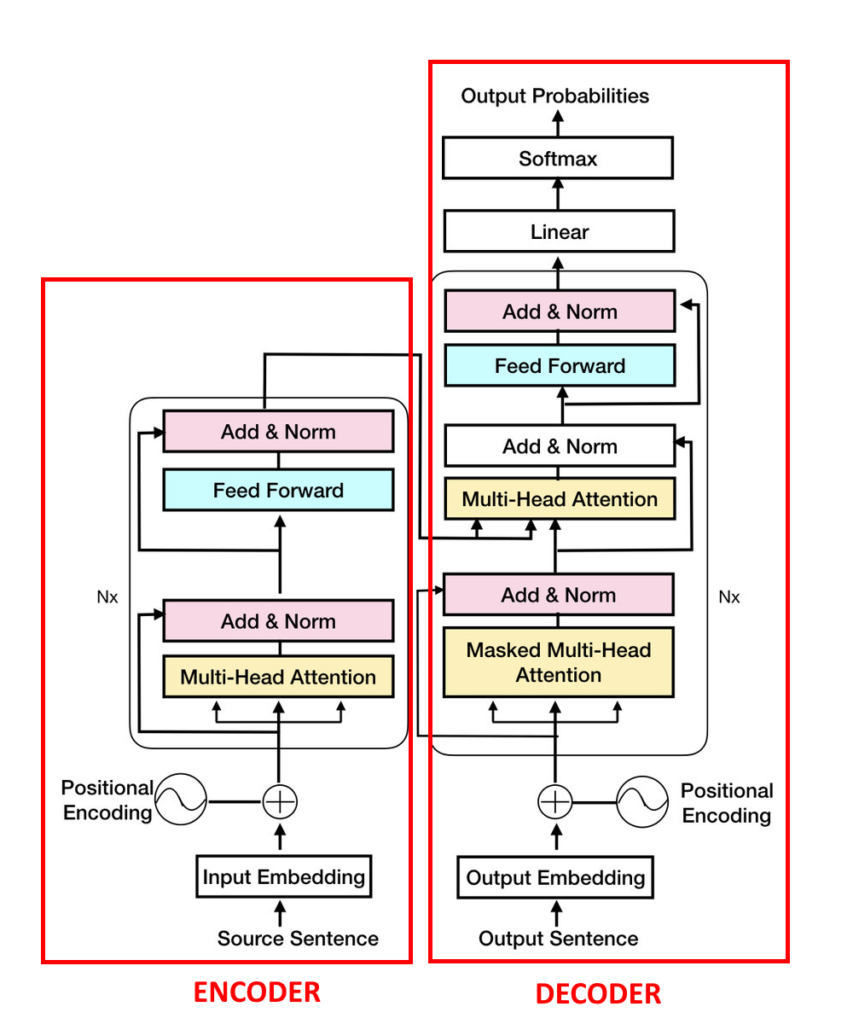
\includegraphics[width=0.60\textwidth]{imaxes/2_Transformer.png}
  \caption[La Arquitectura de los Transformers]{La Arquitectura de los Transformers. \textit{Fuente: \cite{vaswani2023attention}}}
  \label{fig:2_Transformer}
\end{figure}


\newpage
\subsubsection{Enfoque de Fine-Tuning}
\label{subsubsec:enfoquefinetuning}

Fine-Tuning, también conocido como Ajuste Fino \cite{IBM_Fine}, es una práctica frecuente en el ámbito del aprendizaje automático, especialmente en el \acrshort{NLP}. Dentro del contexto de los \acrshort{LLMs}, como \acrshort{GPT}-3 o \acrshort{LLaMA}, este enfoque consiste en modificar los parámetros de un modelo previamente entrenado con una gran cantidad de datos, utilizando información específica de la tarea a resolver.

Por lo tanto, consiste en volver a entrenar únicamente algunas secciones del modelo, por lo general las capas finales o algunas capas específicas, dejando las capas iniciales sin cambios. Esto posibilita que el modelo preentrenado mantenga el conocimiento general adquirido en el preentrenamiento inicial, mientras se ajusta a la tarea específica para la cual está siendo adaptado.

En el caso de la generación automática de código, se podría usar un modelo de lenguaje grande preentrenado, como \acrshort{GPT}-3, y modificarlo con un conjunto de datos específico de ejemplos de código y descripciones en lenguaje natural. El modelo se entrenará para producir código con mayor precisión y coherencia, adaptándose a las especificaciones dadas.

\subsubsection{Enfoque RAG}
\label{subsubsec:enfoquerag}

El \acrfull{RAG} es una técnica que complementa la generación de texto con información de fuentes de datos privadas o propietarias\cite{GobiernoEspana_RAG}. Combina un modelo de recuperación, que está diseñado para buscar grandes \textit{sets} de datos o bases de conocimiento, con un modelo de generación como el \acrfull{LLMs}, que toma esa información y genera una respuesta de texto legible como se muestra en la figura \ref{fig:2_RAG}.

Incrementar la generación de recuperación puede elevar la importancia de una búsqueda al incluir información extra y complementar el conocimiento inicial del entrenamiento de un \acrshort{LLMs}. Esto aumenta la eficacia del gran modelo de lenguaje sin la necesidad de reentrenarlo. Las fuentes de información extra pueden incluir desde datos nuevos en línea no adiestrados por el \acrshort{LLMs} hasta información confidencial interna de compañías o contexto comercial exclusivo.

\bigskip % Deja una línea en blanco

\begin{figure}[hp!]
  \centering
  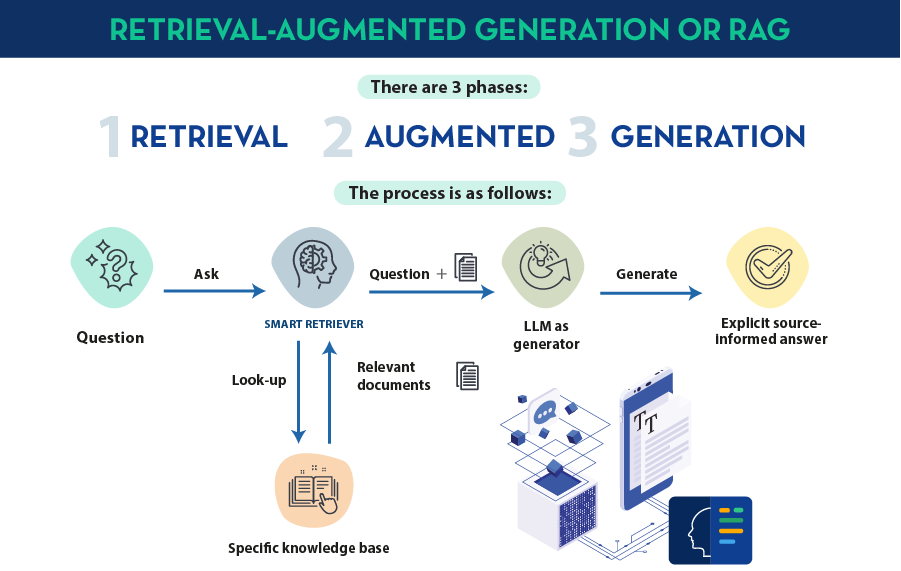
\includegraphics[width=0.75\textwidth]{imaxes/2_RAG.png}
  \caption[Esquema del funcionamiento de un Modelo RAG]{Esquema del funcionamiento de un Modelo RAG. \textit{Fuente: \cite{GobiernoEspana_RAG}}}
  \label{fig:2_RAG}
\end{figure}



